\documentclass[a4paper]{scrartcl}
\usepackage[utf8]{inputenc}
\usepackage{amsmath,amssymb,amsthm}
\usepackage{enumitem,setspace}
\usepackage[usenames,dvipsnames,table]{xcolor}
\usepackage{graphicx}
\DeclareGraphicsExtensions{.pdf,.png,.eps,.jpg}
\usepackage{algorithm2e}
\usepackage{tikz}
\usepackage{float}

% --- math operators ---
\usepackage{mathtools}
\DeclarePairedDelimiter\set{\{}{\}} % use $\set{1, 2, 3}$
\DeclarePairedDelimiter\abs{\lvert}{\rvert}
\DeclarePairedDelimiter\norm{\lVert}{\rVert}
\DeclarePairedDelimiter\ceils{\lceil}{\rceil}
\DeclarePairedDelimiter\floor{\lfloor}{\rfloor}
\def\then{\ensuremath{\Rightarrow}} % =>
\def\iff{\ensuremath{\Leftrightarrow}} % if and only if <=>
\def\to{\ensuremath{\rightarrow}} % ->
\def\ot{\ensuremath{\leftarrow}} % ->
\def\Oh{\ensuremath{\mathcal{O}}} % big O like $\Oh(n)$
% ---
\DeclareMathOperator{\preorder}{preorder}
\DeclareMathOperator{\postorder}{postorder}
\DeclareMathOperator{\depth}{depth}

% --- FILL OUT THESE 3 FIELDS ---
\def\sheetNumber{1}
\def\names{NAMEN} 
\def\sumPoints{20} 

% --- ### BEGIN DOCUMENT ### ---
\begin{document} 

\begin{doublespace} % header
\noindent \textbf{\LARGE{Übungsblatt \sheetNumber}}
\hfill  {\large Punkte: $\boxed{\qquad  /\; \sumPoints}$}\\
{\Large \textbf{Fortgeschrittene Algorithmen (Wintersemester 2022/23)}\\
Bearbeitet von: \textbf{\names}\\
\today}
\end{doublespace}


\section*{Aufgabe 1}
\newpage
\section*{Aufgabe 2}
a)
Suffixbaum zu S = \texttt{mississippi\$}:
\begin{center}
    \begin{figure}[H]
        \resizebox{0.95\textwidth}{!}{
        \tikzset{
        % Set the overall layout of the tree
        level 1/.style = {level distance=3.5cm, sibling distance=5cm},
        level 2/.style = {level distance=3.5cm, sibling distance=3.5cm},
        level 3/.style = {level distance=3.5cm, sibling distance=2.5cm},
        % Define styles for bags and leafs
        bag/.style = {circle, draw, thick, text width=4cm, text centered, inner sep=2pt},
        end/.style = {minimum width=6pt, fill, inner sep=0pt} 
        }
        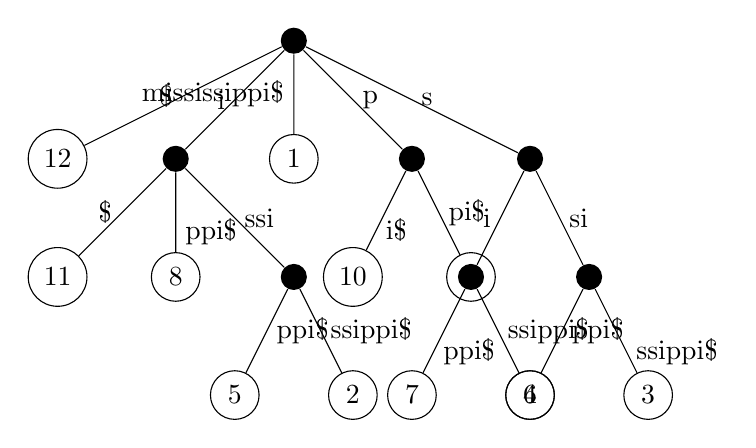
\begin{tikzpicture}[grow=down]
            \tikzset{frontier/.style={distance from root=150pt}}
            
            \node[circle, fill] {}
            child {
                    node[circle, draw] {12}
                    edge from parent node[left] {\$}
                }
                child {
                    node[circle, fill] {}
                    child{
                        node[circle, draw] {11}
                        edge from parent node[left] {\$}
                    }
                    child{
                        node[circle, draw] {8}
                        edge from parent node[right, near end] {ppi\$}
                    }
                    child {
                        node[circle, fill] {}
                        child{
                            node[circle, draw] {5}
                            edge from parent node[right] {ppi\$}
                        }
                        child{
                            node[circle, draw] {2}
                            edge from parent node[right] {ssippi\$}
                        }
                        edge from parent node[right] {ssi}
                    }
                    edge from parent node[left] {i}
                }
                child {
                    node[circle, draw] {1}
                    edge from parent node[left] {mississippi\$}
                }
                child {
                    node[circle, fill] {}
                    child{
                        node[circle, draw] {10}
                        edge from parent node[right, near end] {i\$}
                    }
                    child{
                        node[circle, draw] {9}
                        edge from parent node[right] {pi\$}
                    }
                    edge from parent node[right] {p}
                }
                child {
                    node[circle, fill] {}
                    child{
                        node[circle, fill] {}
                        child{
                            node[circle, draw] {7}
                            edge from parent node[right, near end] {ppi\$}
                        }
                        child{
                            node[circle, draw] {4}
                            edge from parent node[right] {ssippi\$}
                        }
                            edge from parent node[left] {i}
                    }
                    child{
                        node[circle, fill] {}
                        child{
                            node[circle, draw] {6}
                            edge from parent node[right] {ppi\$}
                        }
                        child{
                            node[circle, draw] {3}
                            edge from parent node[right, near end] {ssippi\$}
                        }
                    edge from parent node[right] {si}
                    }
                    edge from parent node[right] {s}
                }
                
                
                ;
        \end{tikzpicture}
        }
    \end{figure}
\end{center}
Suffixarray zu S = \texttt{mississippi\$}:

\begin{equation}
    \def\arraystretch{1.5}
    \begin{array}{|c|c|c|c|c|c|c|c|c|c|c|c|}
        \hline
        12 & 11 & 8 & 5 & 2 & 1 & 10 & 9 & 7 & 4 & 6 & 3 \\
        \hline
        \rotatebox{-90}{\$} & \rotatebox{-90}{i\$} & \rotatebox{-90}{ippi\$} &
         \rotatebox{-90}{issippi\$} & \rotatebox{-90}{ississippi\$} & \rotatebox{-90}{mississippi\$}  & 
         \rotatebox{-90}{pi\$} & \rotatebox{-90}{ppi\$} & \rotatebox{-90}{sippi\$} & 
         \rotatebox{-90}{sissippi\$} & \rotatebox{-90}{ssippi\$} & \rotatebox{-90}{ssissippi\$} \\
    \end{array}
\end{equation}

b) Der Suffixbaum wird erweitert, indem für jeden Knoten die Anzahl der Blätter in seinem Teilbaum gespeichert wird. Dies kann in einer Nach-Ordnung Traversierung des Baumes in linearer Zeit durchgeführt werden.
 Anschließend kann die Anzahl der Vorkommen eines Musters P durch eine Suche im Suffixbaum in $\Oh(m\log\abs\sum)$ Zeit bestimmt werden, indem
man das Muster P von der Wurzel ausgehend im Baum sucht. Findet man das Muster, so gibt die gespeicherte Anzahl der Blätter im Teilbaum des 
Endknotens die Anzahl der Vorkommen von P in S an. Falls das Muster nicht gefunden wird, so kommt es 0 mal vor.

\section*{Aufgabe 3}

\section*{Aufgabe 4}


% -- code for figures
% \begin{figure}[htb]
% \centering
% \includegraphics{filename} % use option [width=\linewidth] to change size to linewidth (or 0.6\linewidth for example)
% \label{fig:name}
% \end{figure}


\end{document}
% --- ### END DOCUMENT ### ---